\documentclass[conference,letterpaper]{IEEEtran}
\usepackage[T1]{fontenc}
\usepackage{cite}
\usepackage{amsmath}
\usepackage{graphicx}
\usepackage{booktabs}
\usepackage{times}
\graphicspath{{figures/}}

\begin{document}

\title{Reference-Normalized Diagnosis of Parametric Faults in 6T SRAM Across Operating Corners}
\author{\IEEEauthorblockN{Anonymous submission}}
\maketitle

\begin{abstract}
Process, voltage, and temperature variation can obscure the electrical signatures of parametric faults in six-transistor static random-access memory. We evaluate matched-reference normalization using 1,350 simulated cell observations across 45 operating corners, covering a healthy class and four defect classes. In leave-one-corner-out evaluation, the normalized feature set raises Random Forest accuracy from 75.11 to 99.33 percent and worst-corner accuracy from 50.00 to 90.00 percent. A controlled comparison using the same five measurements and the same healthy reference gives 76.74 percent with unnormalized target and reference inputs and 99.11 percent with their ratios. At a fixed access-path open, normalization reduces cross-corner variation in write delay and bitline swing. Joint holdout of operating corner and interior fault-parameter levels gives 99.11 percent accuracy on 450 faulty observations. At the parameter boundary, accuracy on the weakest tested opens is 76.67 percent. The results quantify the benefit and limits of reference normalization within the simulated operating grid.
\end{abstract}

\begin{IEEEkeywords}
Fault diagnosis, machine learning, process-voltage-temperature variation, reference normalization, static noise margin, static random-access memory.
\end{IEEEkeywords}

\section{Introduction}

Device and operating-condition variation affect the stability and timing of static random-access memory (SRAM) \cite{mukhopadhyay2005modeling,mukhopadhyay2007memories}. These shifts complicate diagnosis because a change in access time or read margin can arise from a defect, a different operating corner, or both. In this study, 1,009 of 1,080 resistive-open and threshold-shift observations pass the four simulated hold, write, read-stability, and bistability checks. Electrical measurements provide additional information for distinguishing configurations with the same screening outcomes.

March-based tests address defined classes of functional memory faults \cite{vandegoor1993march,vandegoor2000functional,hamdioui2003dynamic}. Programmable weak-cell screening can target reduced stability margins \cite{pavlov2004sram}. Reference-based analog screening also has precedent. Sabade and Walker \cite{sabade2004comparison} compared differences and ratios of quiescent current across test vectors. Here, each reference comes from a separate healthy simulation at the target's process, supply voltage, and temperature. It provides a baseline for timing, swing, stability, and sampled supply-current measurements. Static noise margin (SNM) is derived from the SRAM butterfly construction \cite{seevinck1987static}.

Machine learning has been applied in semiconductor test and post-silicon diagnosis \cite{makris2018special,amrouch2022machine}. Venkatesan \emph{et al.} \cite{venkatesan2024sram} investigated neural-network diagnosis using simulated SRAM responses and data augmentation. The question here is how much operating-corner variation can be removed before classification by incorporating a healthy reference. We evaluate an automated transistor-level benchmark, compare normalization operators under identical corner splits, and test performance when the operating corner and selected defect parameters are withheld together.

\section{Transistor-Level Simulation Benchmark}

\subsection{Cell and Operating Grid}

The six-transistor (6T) cell in Fig.~\ref{fig:cell} uses generic Level-1 MOSFET models with 180\,nm channel lengths. Transistors $M_1/M_4$ drive $Q_b$, and $M_2/M_3$ drive $Q$. The wordline controls $M_5$ and $M_6$, which connect these storage nodes to their respective bitlines. Pull-up, access, and pull-down widths are 360, 540, and 720\,nm, respectively. The geometric cell ratio is 1.333, and the pull-up ratio is 0.667.

\begin{figure}[!t]
\centering
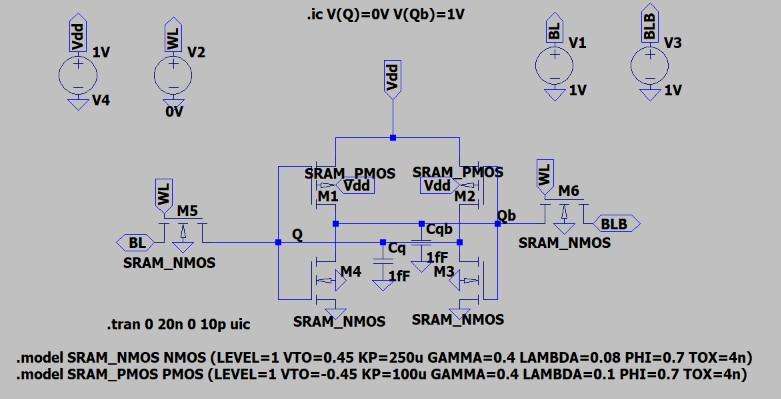
\includegraphics[width=\columnwidth]{6T_SRAM_LTSPICE.jpg}
\caption{Healthy 6T SRAM cell under hold bias. The wordline is low, and the two cross-coupled inverters retain complementary values at $Q$ and $Q_b$.}
\label{fig:cell}
\end{figure}

The process settings are typical-typical (TT), fast-fast (FF), and slow-slow (SS). At TT, the NMOS and PMOS threshold parameters $V_{\mathrm{TO}}$ are $+0.450$ and $-0.450$\,V, and their transconductance parameters $KP$ are 250 and $100\,\mu$A/V$^2$. FF scales $|V_{\mathrm{TO}}|$ and $KP$ by 0.90 and 1.10, respectively. SS applies 1.10 and 0.90. These are global model-card perturbations. Three supply voltages (0.9, 1.0, and 1.1\,V) and five temperatures ($-40$, 0, 27, 75, and $125\,^{\circ}$C) give 45 process-voltage-temperature (PVT) corners.

\subsection{Fault Injection and Batch Execution}

At each corner, the generator instantiates one healthy cell and the 29 single-defect configurations in Table~\ref{tab:faults}. For an open, a series resistor is placed on the bitline side of one access transistor. A bridge is a shunt between the two storage nodes. Threshold shifts increase the magnitude of $V_{\mathrm{TO}}$ on either all four storage devices or both access devices. For PMOS, the threshold parameter becomes more negative. The shifts represent discrete electrical perturbations.

\begin{table}[!t]
\caption{Injected Configurations per Operating Corner}
\label{tab:faults}
\centering
\footnotesize
\setlength{\tabcolsep}{4pt}
\begin{tabular}{@{}llr@{}}
\toprule
Class & Parameter values & Rows \\
\midrule
Healthy & Unmodified cell & 1 \\
Access-path open & 0.2, 0.5, 1, 2, 5, 10\,k$\Omega$ per site & 12 \\
Storage-node bridge & 0.5, 1, 2, 5, 10\,k$\Omega$ & 5 \\
Storage threshold shift & 5, 10, 15, 20, 25, 30\% & 6 \\
Access threshold shift & 5, 10, 15, 20, 25, 30\% & 6 \\
\bottomrule
\end{tabular}
\end{table}

The Python harness composes operation-specific netlists from each cell and dispatches independent LTspice jobs through a worker pool. Each configuration is evaluated with hold, write 1, write 0, read 1, read 0, and two direct-current (DC) sweeps for hold and read SNM. This produces 1,350 configuration--corner observations from 9,450 target runs (6,750 transient and 2,700 DC). The dedicated healthy reference at each corner adds seven runs, bringing the total to 9,765. Reference and healthy target decks use the same deterministic circuit settings.

\subsection{Electrical Measurements and SNM Extraction}

Write delay is measured from the wordline's 50\% rise to the storage-node crossing at half the supply. Sense delay uses the same start point and ends at the first 100\,mV bitline differential. The swing feature uses a fixed 2.15\,ns strobe. At TT, 1.0\,V, and $27\,^{\circ}$C the stored healthy row gives 60.2\,ps mean write delay, 60.0\,ps mean sense delay, and 224.8\,mV mean swing. Standby current is sampled at 20\,ns. Read bump measures the excursion on the storage node holding zero.

For SNM, the feedback loop is opened in the DC testbenches to generate the voltage transfer characteristics (VTCs) $f$ and $g$ of the two inverter branches. The input is swept in 1\,mV steps. The extraction searches for the largest axis-aligned square in each butterfly lobe using piecewise-linear interpolation. For a candidate position $t$ and side $s$, the two lobes use the respective constraints
\begin{equation}
  f(g(t)+s)\ge t+s,\qquad g(f(t)+s)\ge t+s .
  \label{eq:square}
\end{equation}
The smaller of the two maximum sides is the SNM. The search uses 4,001 candidate positions and 50 bisection steps. At the nominal corner, hold and read SNM are 470.06 and 263.69\,mV. Fig.~\ref{fig:butterfly} shows the nominal hold sweep and its extracted squares.

\begin{figure}[!t]
\centering
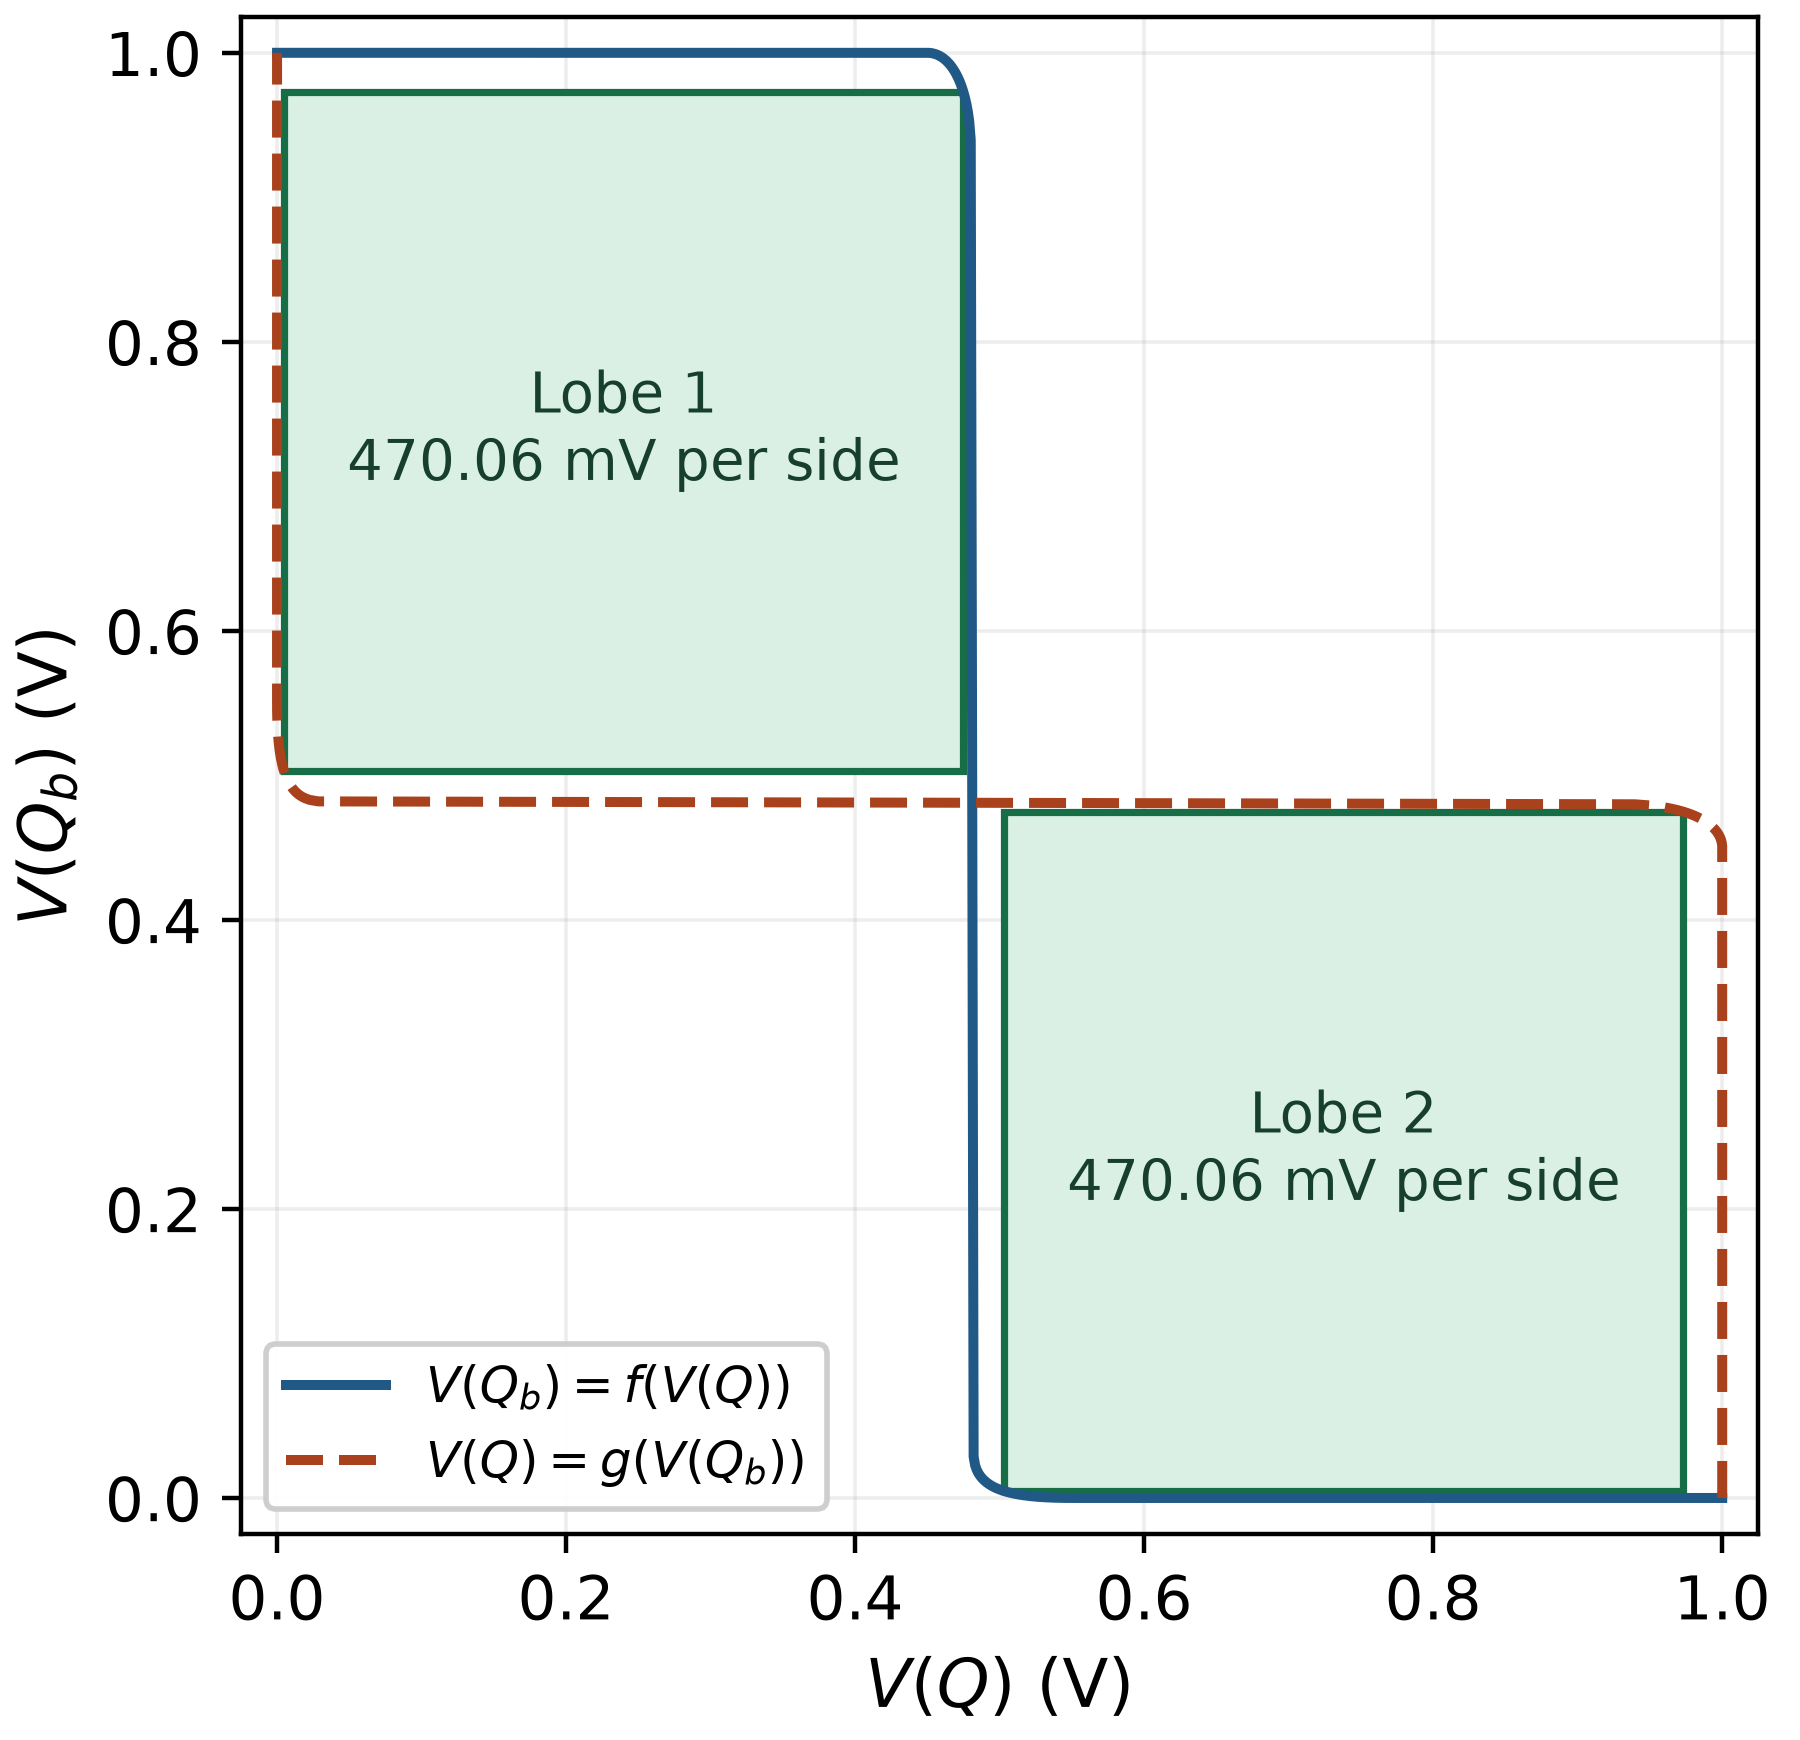
\includegraphics[width=0.94\columnwidth]{snm_butterfly_diagram.png}
\caption{Nominal healthy hold-mode butterfly sweep. Both extracted squares have sides of 470.06\,mV.}
\label{fig:butterfly}
\end{figure}

\subsection{Numerical Status and Retained Observations}

The stored dataset marks 1,327 rows as converged and 23 as nonconverged. Missing measurements can be encoded as finite values, including 20\,ns for unavailable write or sense delays, zero for missing swing or SNM, and ten times the reference for unavailable standby current. These values also carry information about the extraction procedure. At TT, 0.9\,V, and $0\,^{\circ}$C, the healthy row is marked converged despite a rejected read sweep with a 106\,mV nonmonotonic excursion. The stored target read SNM is zero, while the reference estimate used as denominator is approximately 234.7\,mV. A sensitivity check omits the entire affected corner.

\section{Reference-Normalized Features}

\begin{table*}[!t]
\caption{Mean Normalized Ratios and Cross-Corner Dispersion}
\label{tab:dispersion}
\centering
\footnotesize
\newcommand{\cvpair}[3]{\shortstack{$#1$\\$#2\to#3$}}
\begin{tabular*}{0.86\textwidth}{@{\extracolsep{\fill}}lcccc@{}}
\toprule
& \multicolumn{2}{c}{Healthy targets} & \multicolumn{2}{c}{5\,k$\Omega$ access-path open} \\
\cmidrule(lr){2-3}\cmidrule(lr){4-5}
Measurement & All (45) & Marked converged (43) & $M_5$ (43) & $M_6$ (41) \\
\midrule
Sampled standby current & \cvpair{1.200}{197.59}{111.80} & \cvpair{1.000}{139.95}{0.00} & \cvpair{1.000}{148.33}{0.00} & \cvpair{1.000}{142.69}{0.00} \\
\addlinespace
Write delay & \cvpair{1.005}{18.30}{3.49} & \cvpair{1.000}{18.53}{0.00} & \cvpair{1.311}{15.05}{3.66} & \cvpair{1.382}{17.28}{2.50} \\
\addlinespace
Bitline swing & \cvpair{1.000}{38.50}{0.00} & \cvpair{1.000}{38.83}{0.00} & \cvpair{0.978}{36.38}{2.28} & \cvpair{0.978}{37.01}{2.30} \\
\addlinespace
Hold SNM & \cvpair{1.000}{12.40}{0.00} & \cvpair{1.000}{12.31}{0.00} & \cvpair{1.000}{12.49}{0.00} & \cvpair{1.000}{12.62}{0.00} \\
\addlinespace
Read SNM & \cvpair{0.978}{22.10}{15.25} & \cvpair{0.977}{22.26}{15.61} & \cvpair{0.975}{22.54}{15.65} & \cvpair{0.974}{22.74}{16.04} \\
\bottomrule
\end{tabular*}
\par\smallskip
\parbox{0.86\textwidth}{Each cell gives the mean ratio above the raw and normalized CVs (\%). CV is $100s/\bar{x}$, with sample standard deviation $s$ using $n-1$. Parentheses give corner counts. Both open subsets use rows marked converged.}
\end{table*}

Let $x_{ijc}$ be measurement $j$ for target $i$ at corner $c$, and let $h_{jc}$ be that measurement for the simulated healthy reference. The five base measurements are sampled standby current, write delay, bitline swing, hold SNM, and read SNM. For each, the stored normalized feature is
\begin{equation}
  z_{ijc} = \frac{x_{ijc}}{\max(h_{jc},\,\delta_j)} ,
  \label{eq:ratio}
\end{equation}
where the floors $\delta_j$ are $10^{-4}\,\mu$A, 1\,ps, 1\,mV, and 0.05\,V for each SNM. Three further ratios use target measurements: sense-to-write delay, read-to-hold SNM, and swing-to-supply voltage. The first two internal ratios floor the denominators at 1\,ps and $10^{-4}$\,V. For a response of the form $a(c)b(i)$, dividing by a matched reference cancels the shared factor $a(c)$ when the denominator floor is inactive. Interactions between the defect and the operating condition can leave residual variation.

Table~\ref{tab:dispersion} reports normalized means and sample coefficients of variation (CVs), computed on the same rows for each raw and normalized pair. The fixed open measures dispersion in the presence of a defect. Across the 43 converged $M_5$ observations, write-delay CV falls from 15.05\% to 3.66\% and swing CV from 36.38\% to 2.28\%. Across 41 $M_6$ observations, the corresponding changes are 17.28\% to 2.50\% and 37.01\% to 2.30\% (Fig.~\ref{fig:spread}). The mean write-delay ratios are 1.311 and 1.382, respectively, and the mean swing ratio is 0.978 at each site.

The healthy target and reference have the same deterministic settings. A healthy ratio of one is therefore expected when both extractions succeed and use the same value. The rejected read sweep accounts for the single zero among the 45 healthy read-SNM ratios and for their entire normalized CV of 15.25\%. Omitting this corner gives a mean normalized read SNM of 0.998 at both open sites, with CVs of 1.00\% for $M_5$ and 1.03\% for $M_6$.

\begin{figure}[!t]
\centering
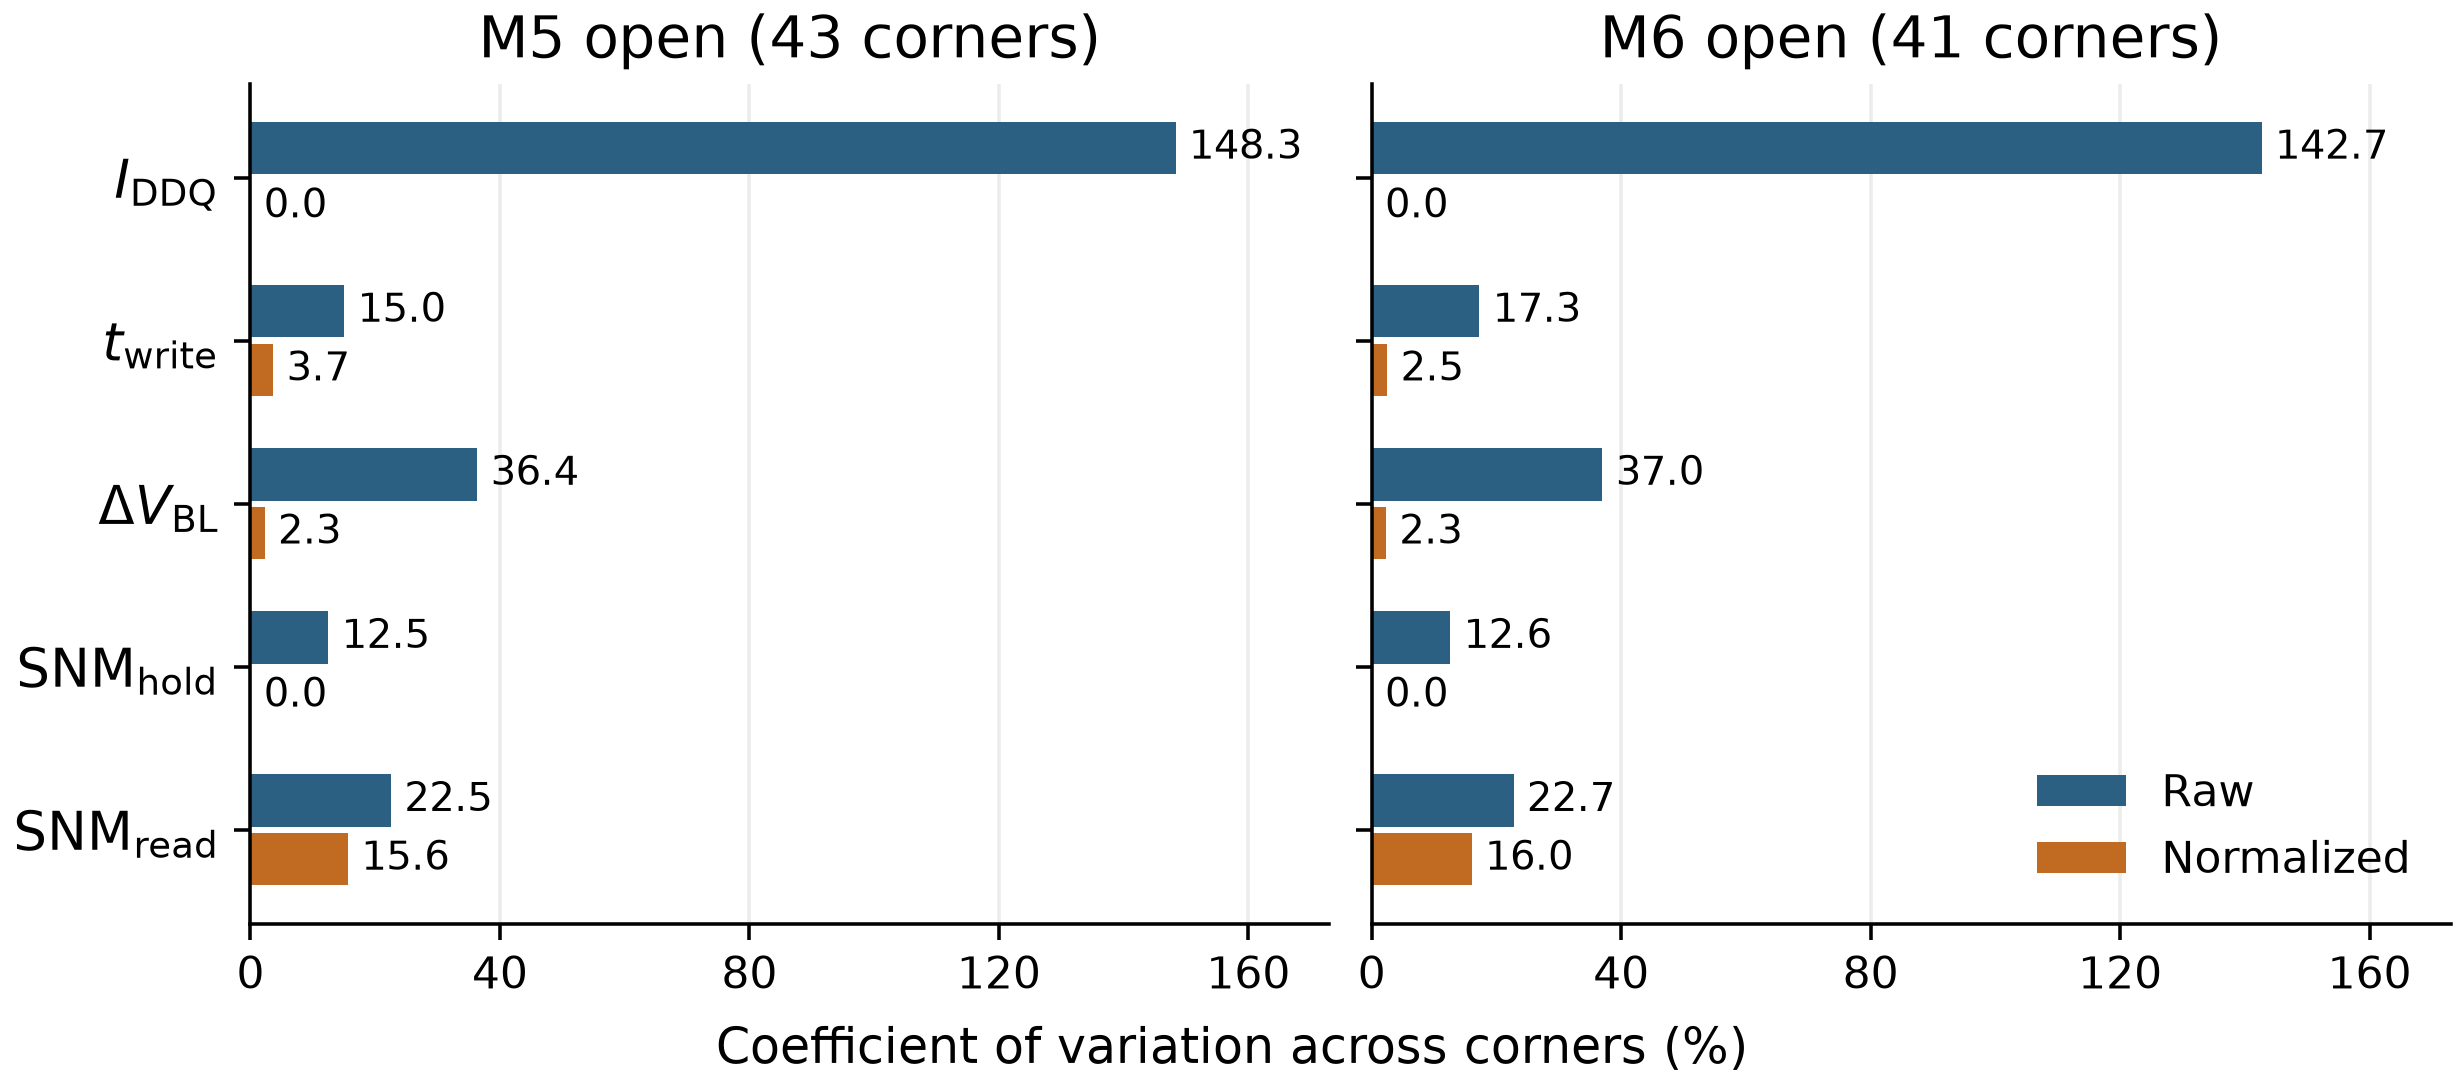
\includegraphics[width=\columnwidth]{fig1_feature_dispersion_comparison.png}
\caption{Cross-corner dispersion for a 5\,k$\Omega$ open on $M_5$ and $M_6$, using 43 and 41 rows marked converged, respectively.}
\label{fig:spread}
\end{figure}

\section{Cross-Corner Evaluation}

\begin{figure*}[!t]
\centering
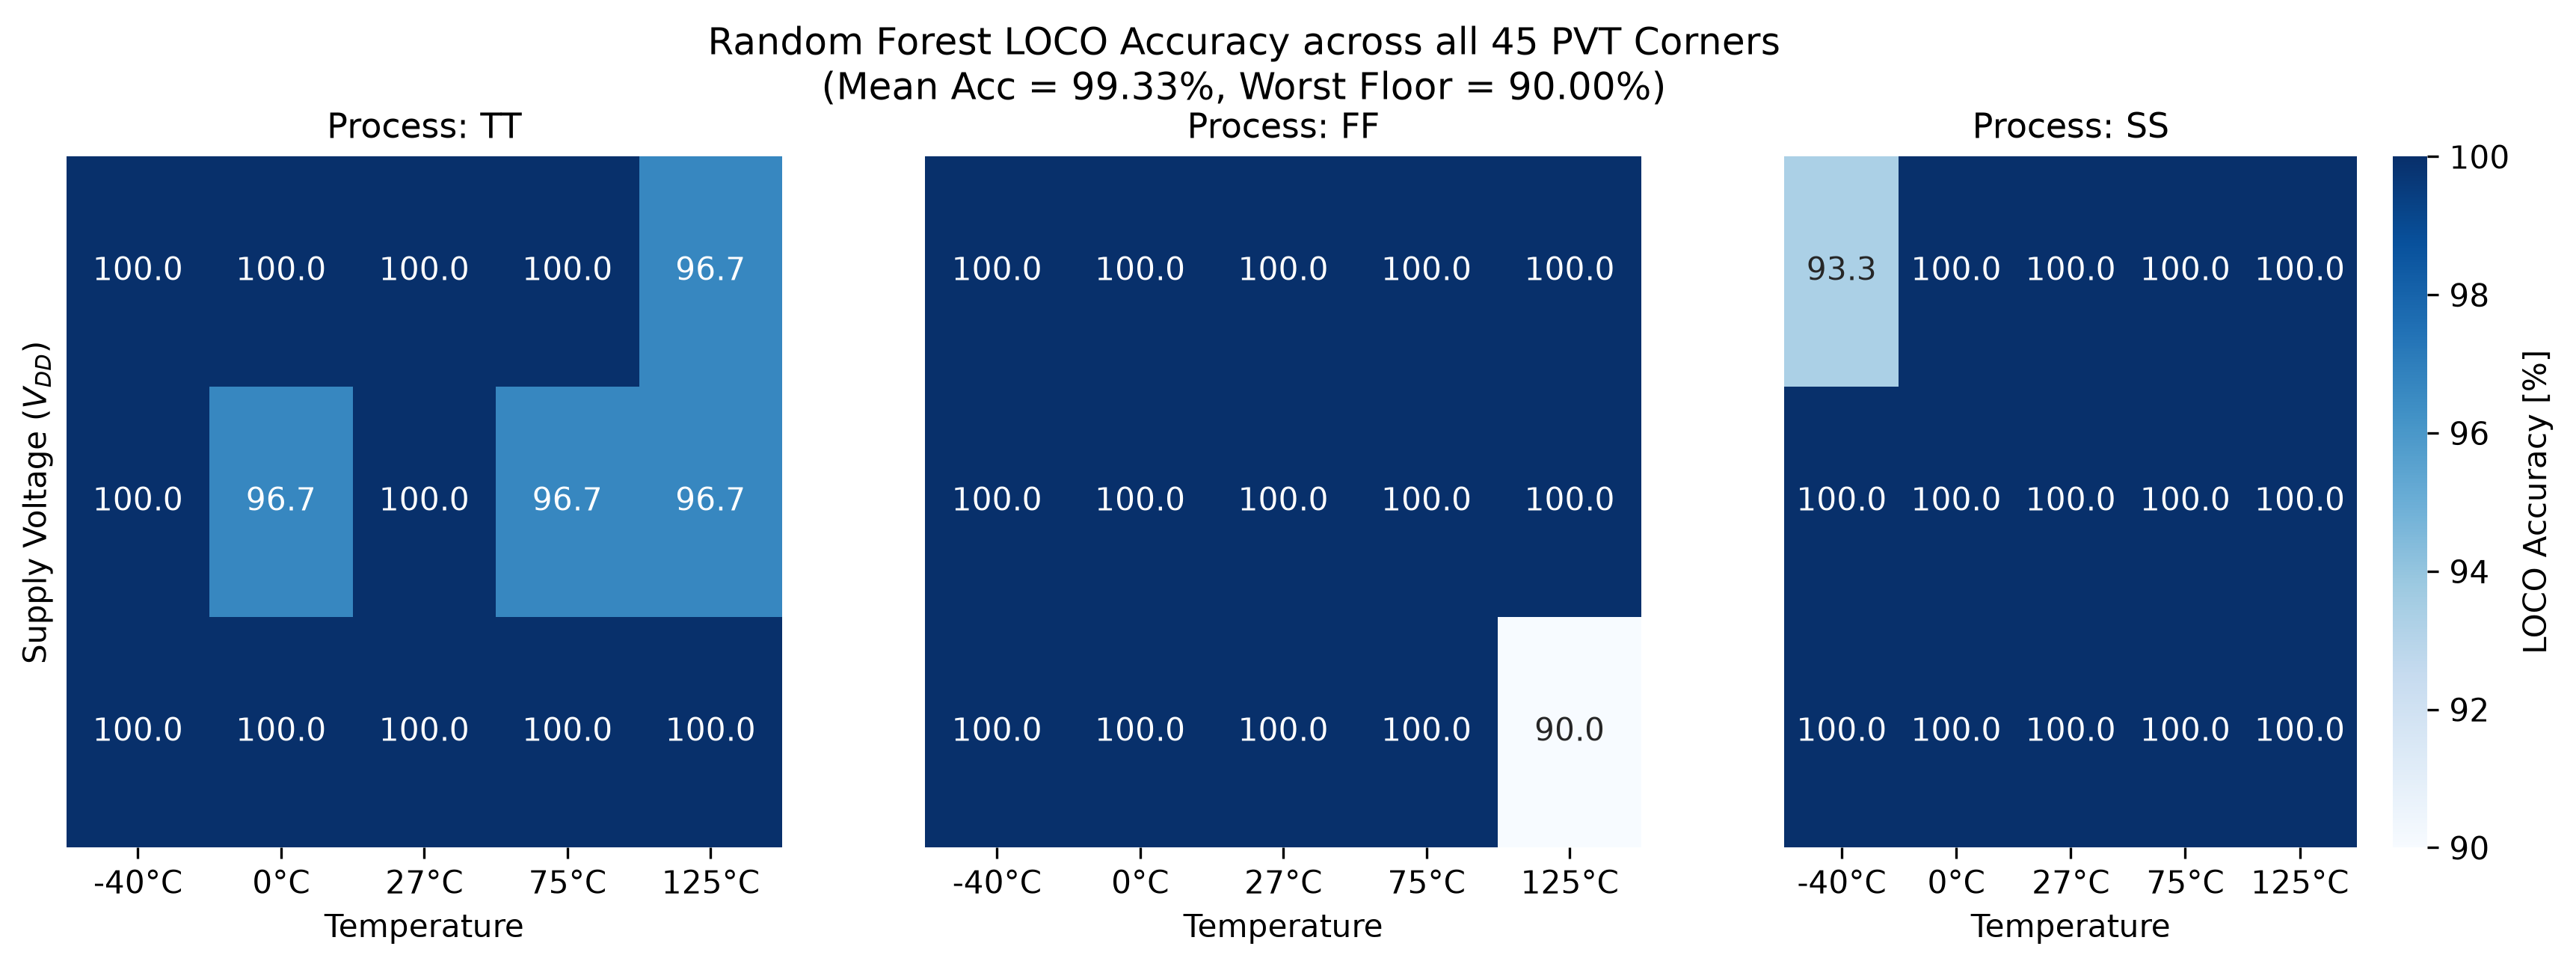
\includegraphics[width=0.91\textwidth]{fig3_rf_pvt_corner_heatmap.png}
\caption{Normalized RF accuracy at each of the 45 held-out operating corners. Rows in each process panel correspond to 0.9, 1.0, and 1.1\,V from top to bottom.}
\label{fig:corners}
\end{figure*}

\subsection{Protocol and Classifier Results}

In leave-one-corner-out (LOCO) evaluation, each of the 45 folds trains on 1,320 observations at 44 corners and tests on the 30 observations at the held-out corner. Its healthy reference is available at test time. The two 12-input sets share four binary functional flags. The raw set contains the five base measurements plus peak write current, sense delay, and read bump. The normalized set contains the five reference ratios and three internal ratios.

The scikit-learn \cite{pedregosa2011scikit} classifiers are Random Forest (RF; 100 trees, maximum depth 10), histogram gradient boosting (HistGB; 100 iterations, maximum depth 6), a decision tree (maximum depth 8), and logistic regression (L2 regularization, at most 1,000 iterations). All use seed 42. The logistic regression inputs are unstandardized. Table~\ref{tab:loco} reports pooled accuracy and the minimum accuracy over the 45 folds. Equal fold sizes make pooled accuracy equal to mean fold accuracy. Balanced accuracy is the mean of the class recalls.

\begin{table}[!t]
\caption{LOCO Accuracy Across 45 Corners (\%)}
\label{tab:loco}
\centering
\footnotesize
\setlength{\tabcolsep}{4pt}
\begin{tabular}{@{}lrrrr@{}}
\toprule
& \multicolumn{2}{c}{Pooled} & \multicolumn{2}{c}{Worst corner} \\
\cmidrule(lr){2-3}\cmidrule(lr){4-5}
Classifier & Raw & Norm. & Raw & Norm. \\
\midrule
Random Forest & 75.11 & 99.33 & 50.00 & 90.00 \\
HistGB & 77.56 & 99.41 & 40.00 & 86.67 \\
Decision tree & 73.56 & 98.44 & 36.67 & 63.33 \\
Logistic regression & 80.59 & 86.89 & 60.00 & 60.00 \\
\bottomrule
\end{tabular}
\end{table}

Normalized inputs raise RF pooled accuracy by 24.22 percentage points. The raw RF reaches its 50.00\% floor at TT and SS with 0.9\,V and $-40\,^{\circ}$C. Fig.~\ref{fig:corners} shows the 39 corners that the normalized RF classifies perfectly and the six with errors. The population standard deviation of RF accuracy across folds falls from 14.15 to 1.94 percentage points. Fig.~\ref{fig:confusion} shows the nine errors among 1,350 predictions. Recall is 97.78\% for healthy, 99.63\% for opens, 100.00\% for bridges, 99.26\% for storage shifts, and 98.52\% for access shifts. Healthy recall here describes deterministic matches to the simulated reference. HistGB has the highest pooled accuracy, while RF has the highest worst-corner accuracy among the tested models.

\begin{figure}[!t]
\centering
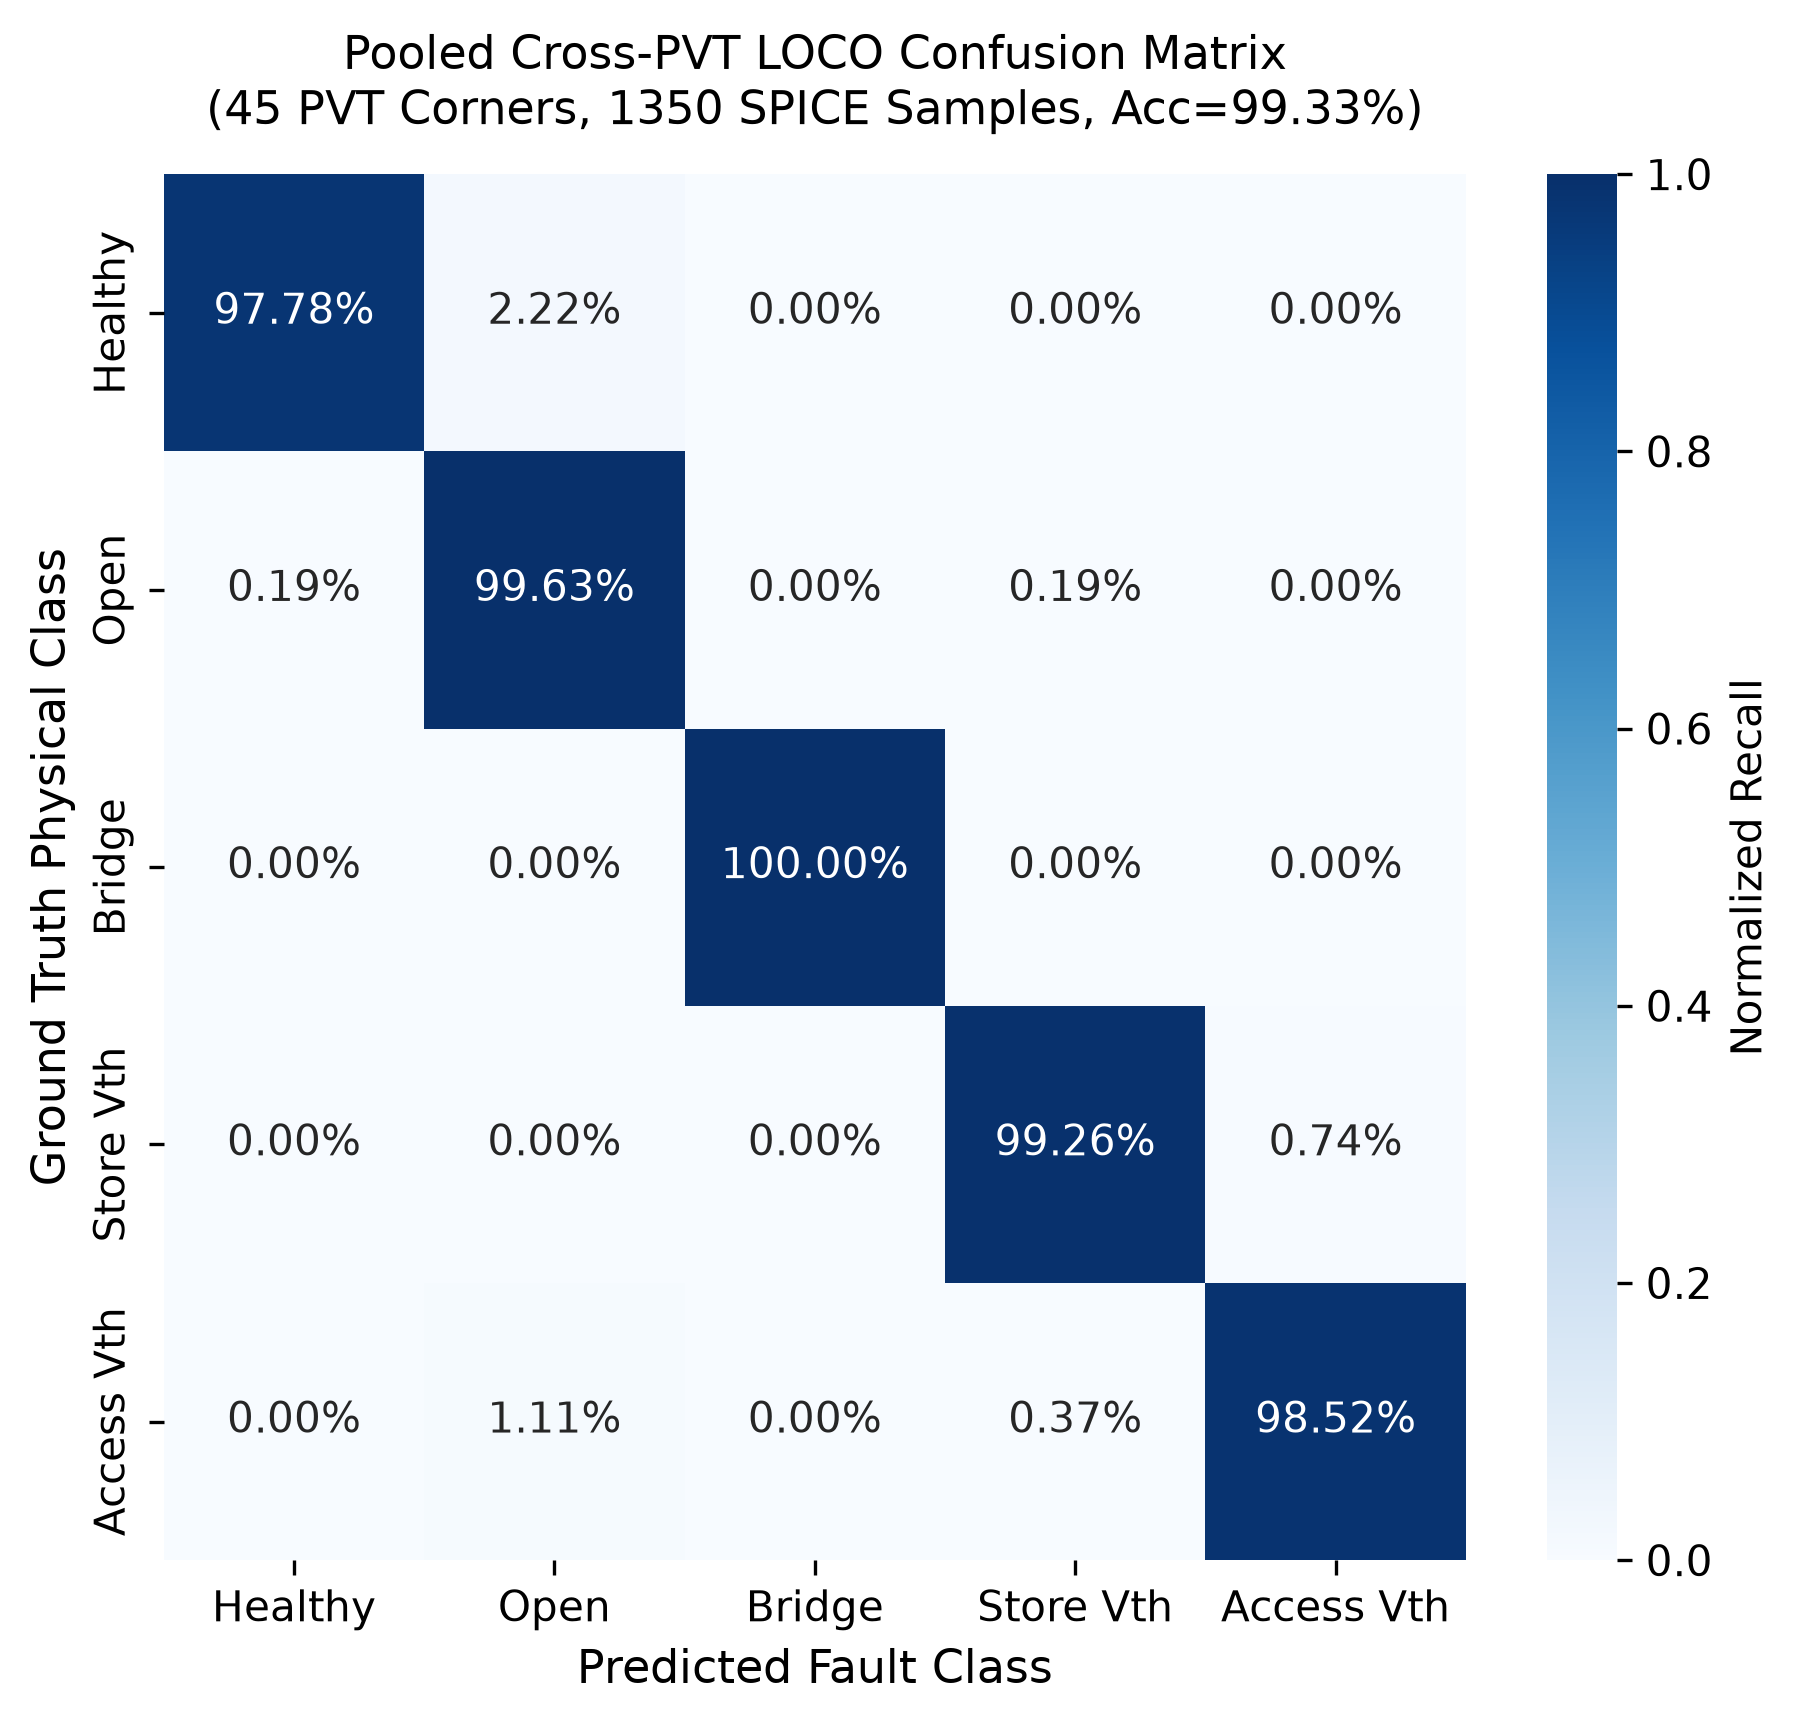
\includegraphics[width=0.98\columnwidth]{fig5_confusion_matrix.png}
\caption{Pooled RF confusion matrix for the normalized ratios and four functional flags. The diagonal contains 1,341 of the 1,350 held-out predictions.}
\label{fig:confusion}
\end{figure}

Excluding the 23 rows marked nonconverged from both training and test sets gives 75.28\% raw and 99.70\% normalized RF accuracy. The flagged read sweep remains in that subset. Removing its entire corner from the full dataset before splitting gives 99.32\% normalized accuracy across 44 corners. In a separate full-grid check, removing the normalized read SNM, read-to-hold SNM ratio, and bistability flag gives 99.56\%.

\subsection{Matched Normalization Controls}

The first five rows of Table~\ref{tab:ablation} use the same base measurements and LOCO splits. The raw-plus-reference control concatenates target and reference measurements. Difference, log-ratio, and ratio use the same healthy observation at the given corner. Thus the healthy row serves as its own reference in this comparison. Each of these controls fixes RF feature sampling at two inputs per split, including the ten-input control. Ratio-based controls replace denominators of magnitude at most $10^{-12}$ with $10^{-12}$ and floor the resulting ratios at that value.

\begin{table}[!t]
\caption{Random Forest Input Controls Under LOCO}
\label{tab:ablation}
\centering
\footnotesize
\setlength{\tabcolsep}{4pt}
\begin{tabular}{@{}lrrr@{}}
\toprule
Inputs & Pooled (\%) & Balanced (\%) & Worst (\%) \\
\midrule
Raw (5) & 73.48 & 62.56 & 36.67 \\
Raw + reference (10) & 76.74 & 64.30 & 36.67 \\
Difference (5) & 98.52 & 98.63 & 80.00 \\
Log-ratio (5) & 99.04 & 99.04 & 83.33 \\
Ratio (5) & 99.11 & 99.11 & 83.33 \\
\midrule
Ratios only (8) & 99.48 & 99.15 & 90.00 \\
Ratios and flags (12) & 99.33 & 99.04 & 90.00 \\
Flags only (4) & 57.70 & 41.59 & 30.00 \\
\bottomrule
\end{tabular}
\end{table}

For this RF, adding raw reference inputs gains 3.26 percentage points over the five raw inputs. Using ratios adds 22.37 points over raw plus reference and 0.59 points over subtraction. A supplementary run of raw plus reference with default square-root feature sampling gives 79.56\%. The eight-ratio and 12-input configurations use the dedicated references and floors in (\ref{eq:ratio}). The eight-ratio result pools all classes and operating conditions. Its electrical inputs can encode functional failures through measured responses and fallback values.

\subsection{Withheld Defect Parameters}

For leave-one-severity-out evaluation, parameter values are ranked in ascending numerical order within each class. Each fold retains healthy rows for training and scores only the faulty rows at the held-out rank (Table~\ref{tab:severity}). At the boundary rank $S_1$, the RF reaches 88.89\% (200/225). The weakest opens at $200\,\Omega$ account for 21 of the 25 errors and score 76.67\% (69/90). The smallest storage and access threshold shifts score 44/45 and 42/45, respectively. For bridges, $S_1$ is the strongest tested bridge because lower resistance increases the coupling. All 45 bridges at that rank are classified correctly.

\begin{table}[!t]
\caption{Leave-One-Severity-Out Results on Faulty Rows}
\label{tab:severity}
\centering
\footnotesize
\setlength{\tabcolsep}{4pt}
\begin{tabular}{@{}lrrl@{}}
\toprule
Rank & Rows & Accuracy (\%) & Position in tested range \\
\midrule
$S_1$ & 225 & 88.89 & Boundary for all classes \\
$S_2$ & 225 & 99.11 & Interior for all classes \\
$S_3$ & 225 & 99.11 & Interior for all classes \\
$S_4$ & 225 & 99.56 & Interior for all classes \\
$S_5$ & 225 & 100.00 & Boundary for bridges only \\
$S_6$ & 180 & 100.00 & Boundary, no bridges \\
\bottomrule
\end{tabular}
\end{table}

For the joint holdout, each fold excludes an entire corner and withholds interior ranks $S_3$ and $S_4$ at all other corners. Test observations are the two withheld ranks at the held-out corner. RF with eight ratios correctly labels 446 of 450 faulty observations (99.11\% pooled accuracy and 99.03\% balanced accuracy). This evaluates interpolation between tested parameter values at a new operating-corner combination.

\section{Interpretation and Sensitivity}

\subsection{Feature Attribution}

Tree SHAP \cite{lundberg2017unified} describes the class-probability outputs of the 12-input RF fitted on all 1,350 observations. Fig.~\ref{fig:shap} averages absolute attributions over observations and all five class outputs. The leading features are normalized write delay (0.0789), normalized swing (0.0776), and normalized read SNM (0.0567). Read SNM still ranks third (0.0613) after excluding the corner with the rejected sweep from both fitting and attribution.

\begin{figure}[!t]
\centering
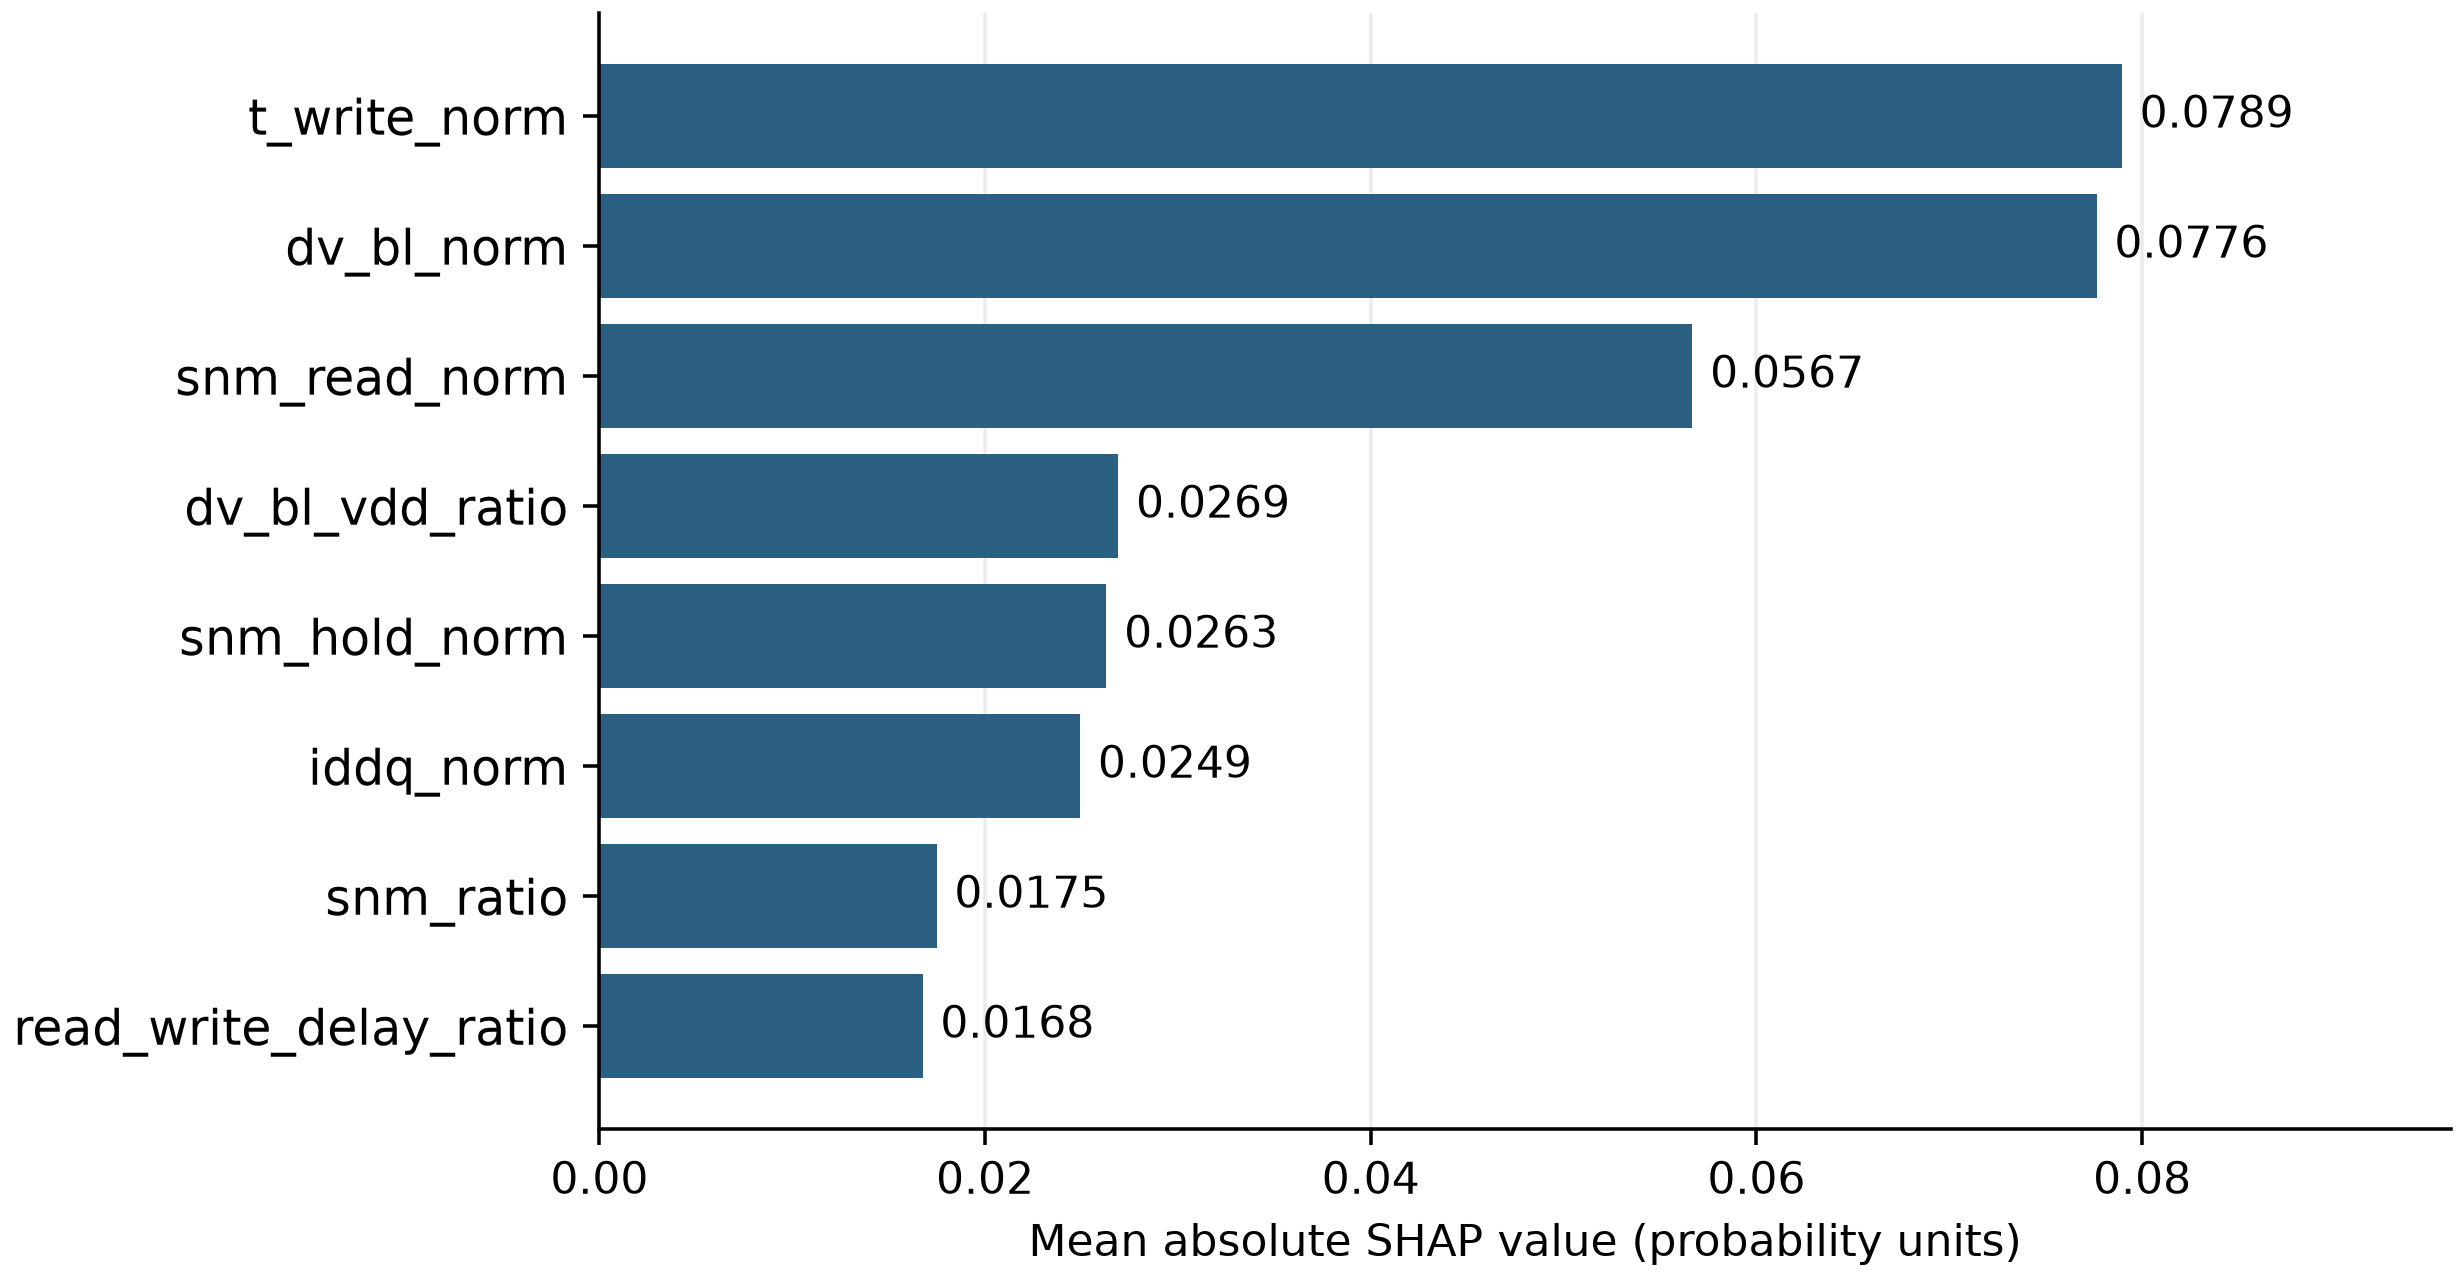
\includegraphics[width=\columnwidth]{fig4_shap_summary.png}
\caption{Global mean absolute Tree SHAP values for the full-data RF, averaged over the five class outputs.}
\label{fig:shap}
\end{figure}

Fig.~\ref{fig:shapclass} shows how these means differ by class output. Normalized swing has the largest attribution for the open class (0.1414). Read SNM and swing lead for access shifts (0.1159 and 0.0906), consistent with the access devices coupling the bitlines and storage nodes during read. Write delay and hold SNM contribute to the storage-shift output (0.1078 and 0.0650). For the bridge output, fallback delays for failed transitions can contribute to the write-delay attribution.

\begin{figure}[!t]
\centering
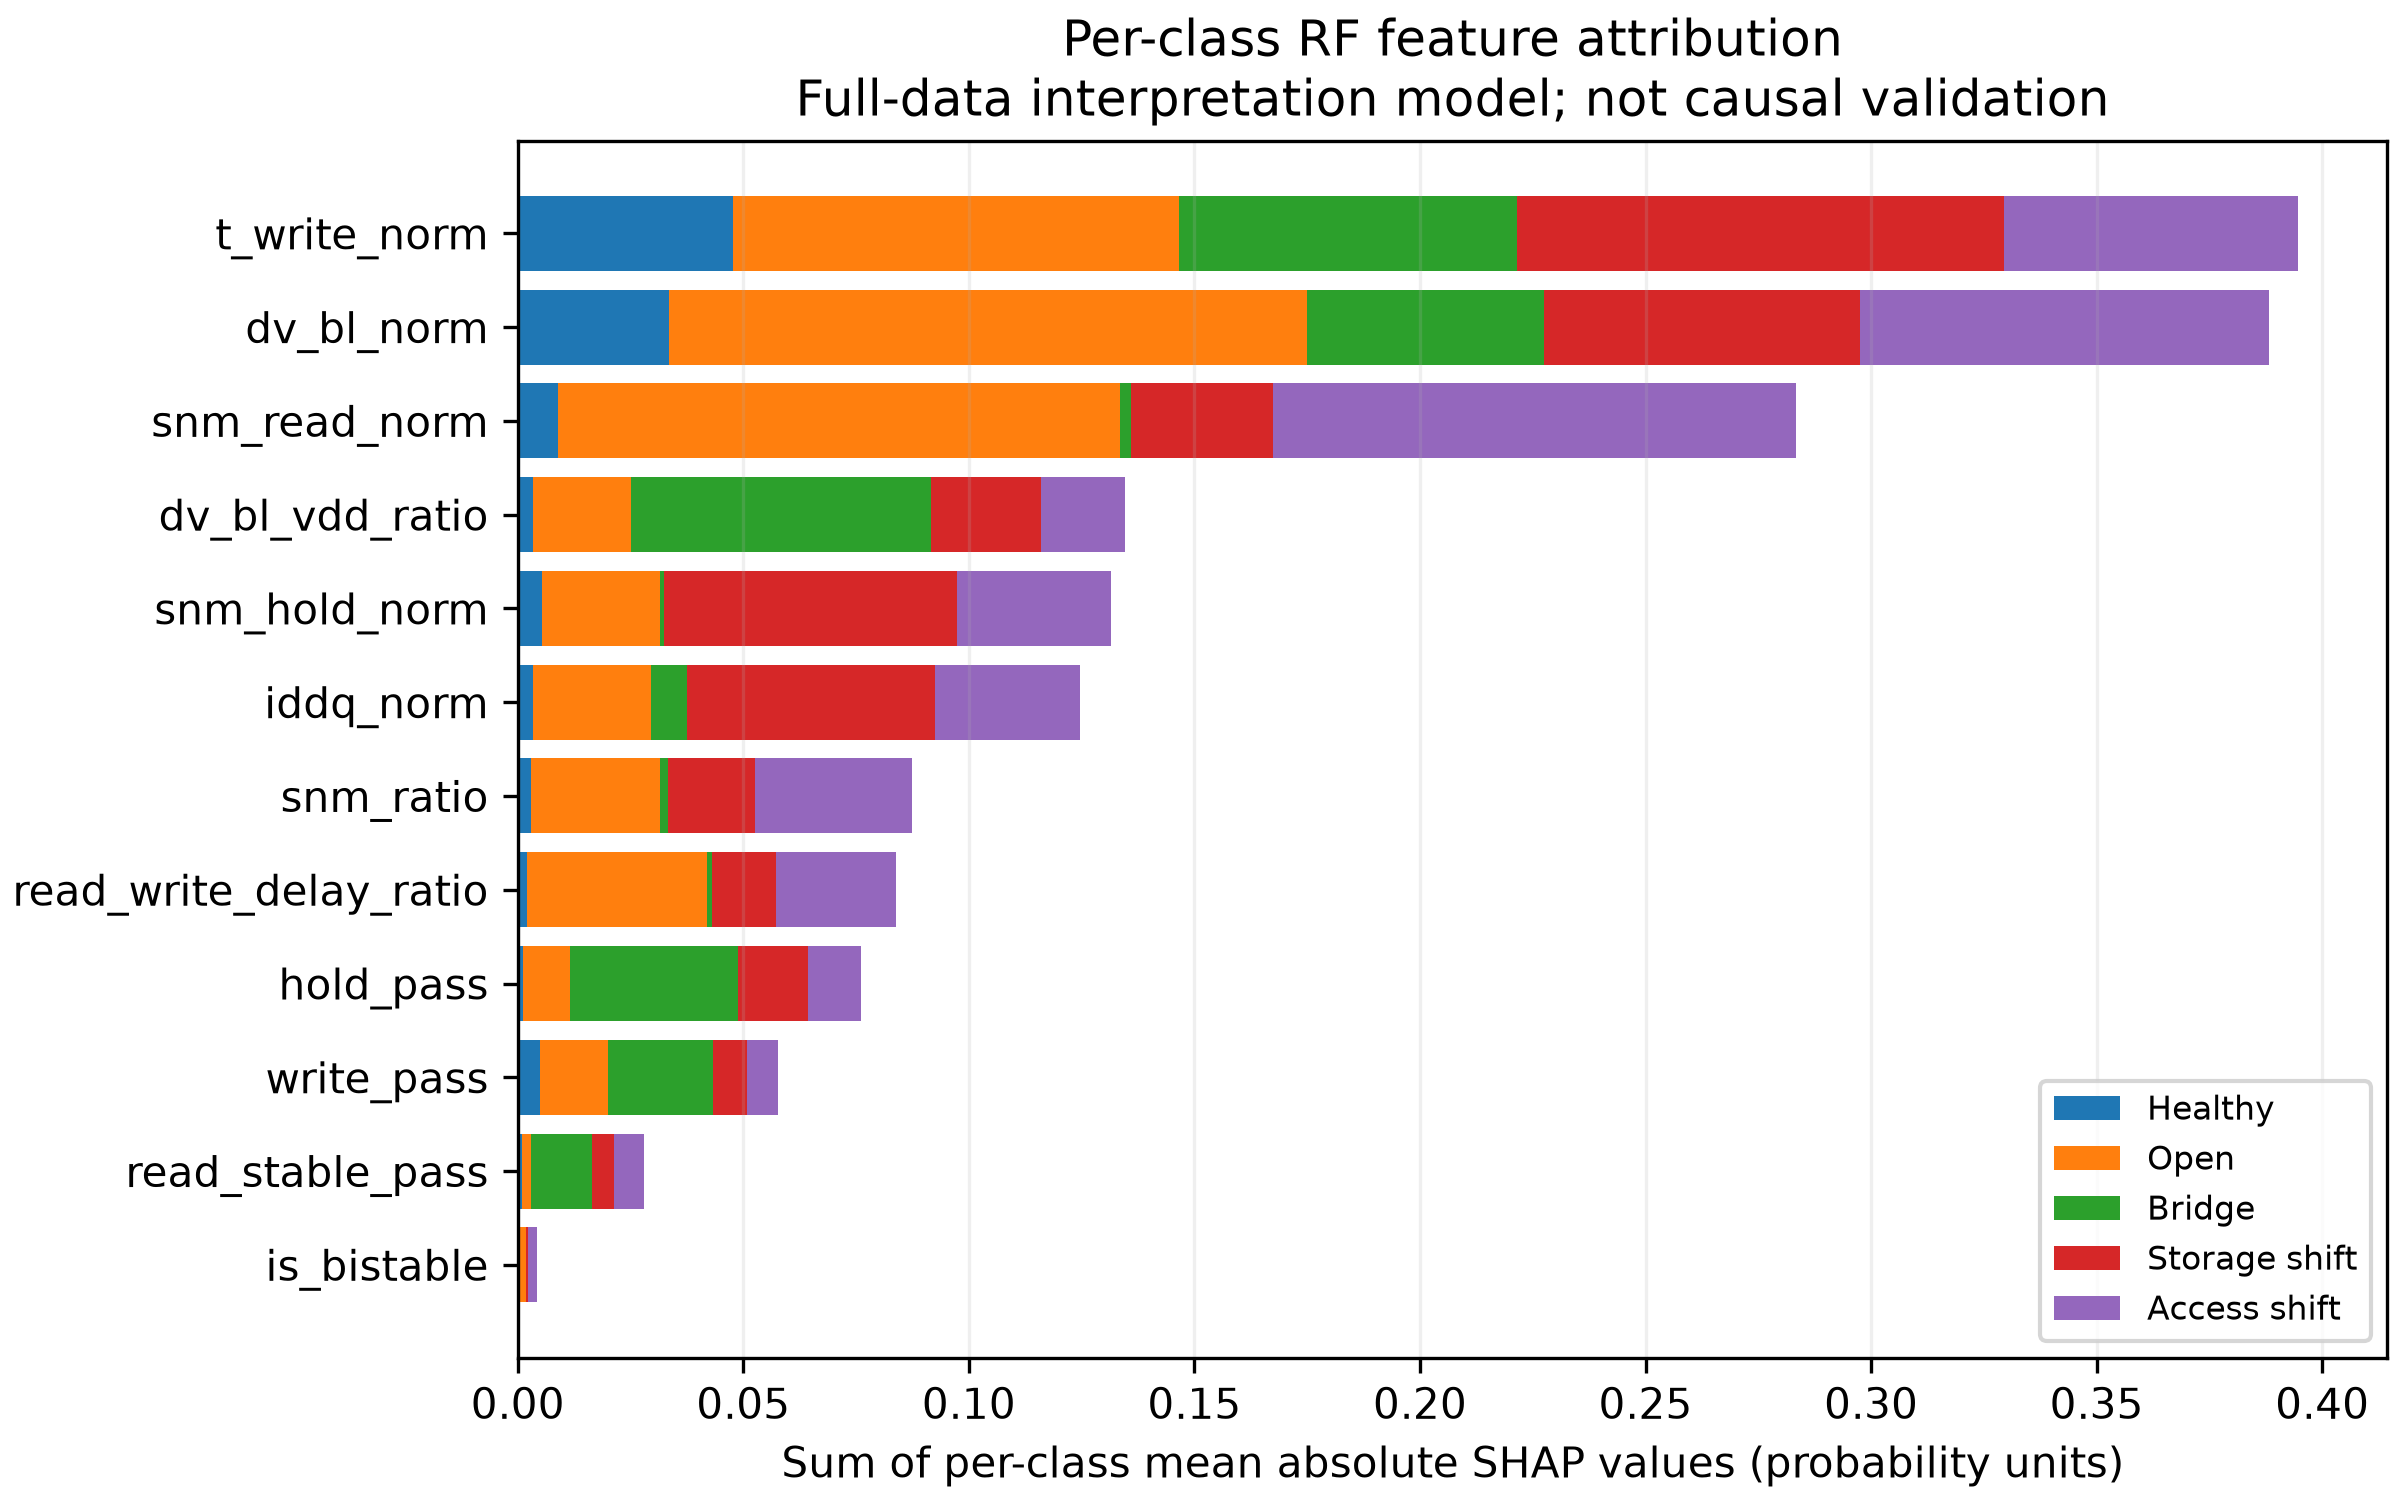
\includegraphics[width=\columnwidth]{fig4b_shap_class_importance.png}
\caption{Mean absolute Tree SHAP values by class output for the full-data RF.}
\label{fig:shapclass}
\end{figure}

\subsection{Feature Noise and Scope}

In a feature-noise check, each row receives one Gaussian multiplier $1+\epsilon_i$, with $\epsilon_i\sim\mathcal{N}(0,\sigma^2)$, shared across all eight ratio inputs. The noisy training and test data are evaluated with refitting at each level. At $\sigma=5\%$, pooled accuracy is 94.22\% and balanced accuracy is 78.11\%. At $\sigma=15\%$, pooled accuracy is 90.67\% and the worst corner falls to 56.67\%. Fig.~\ref{fig:noise} shows the different responses of the three metrics. These results describe one noise realization per level with matched train and test perturbations.

\begin{figure}[!t]
\centering
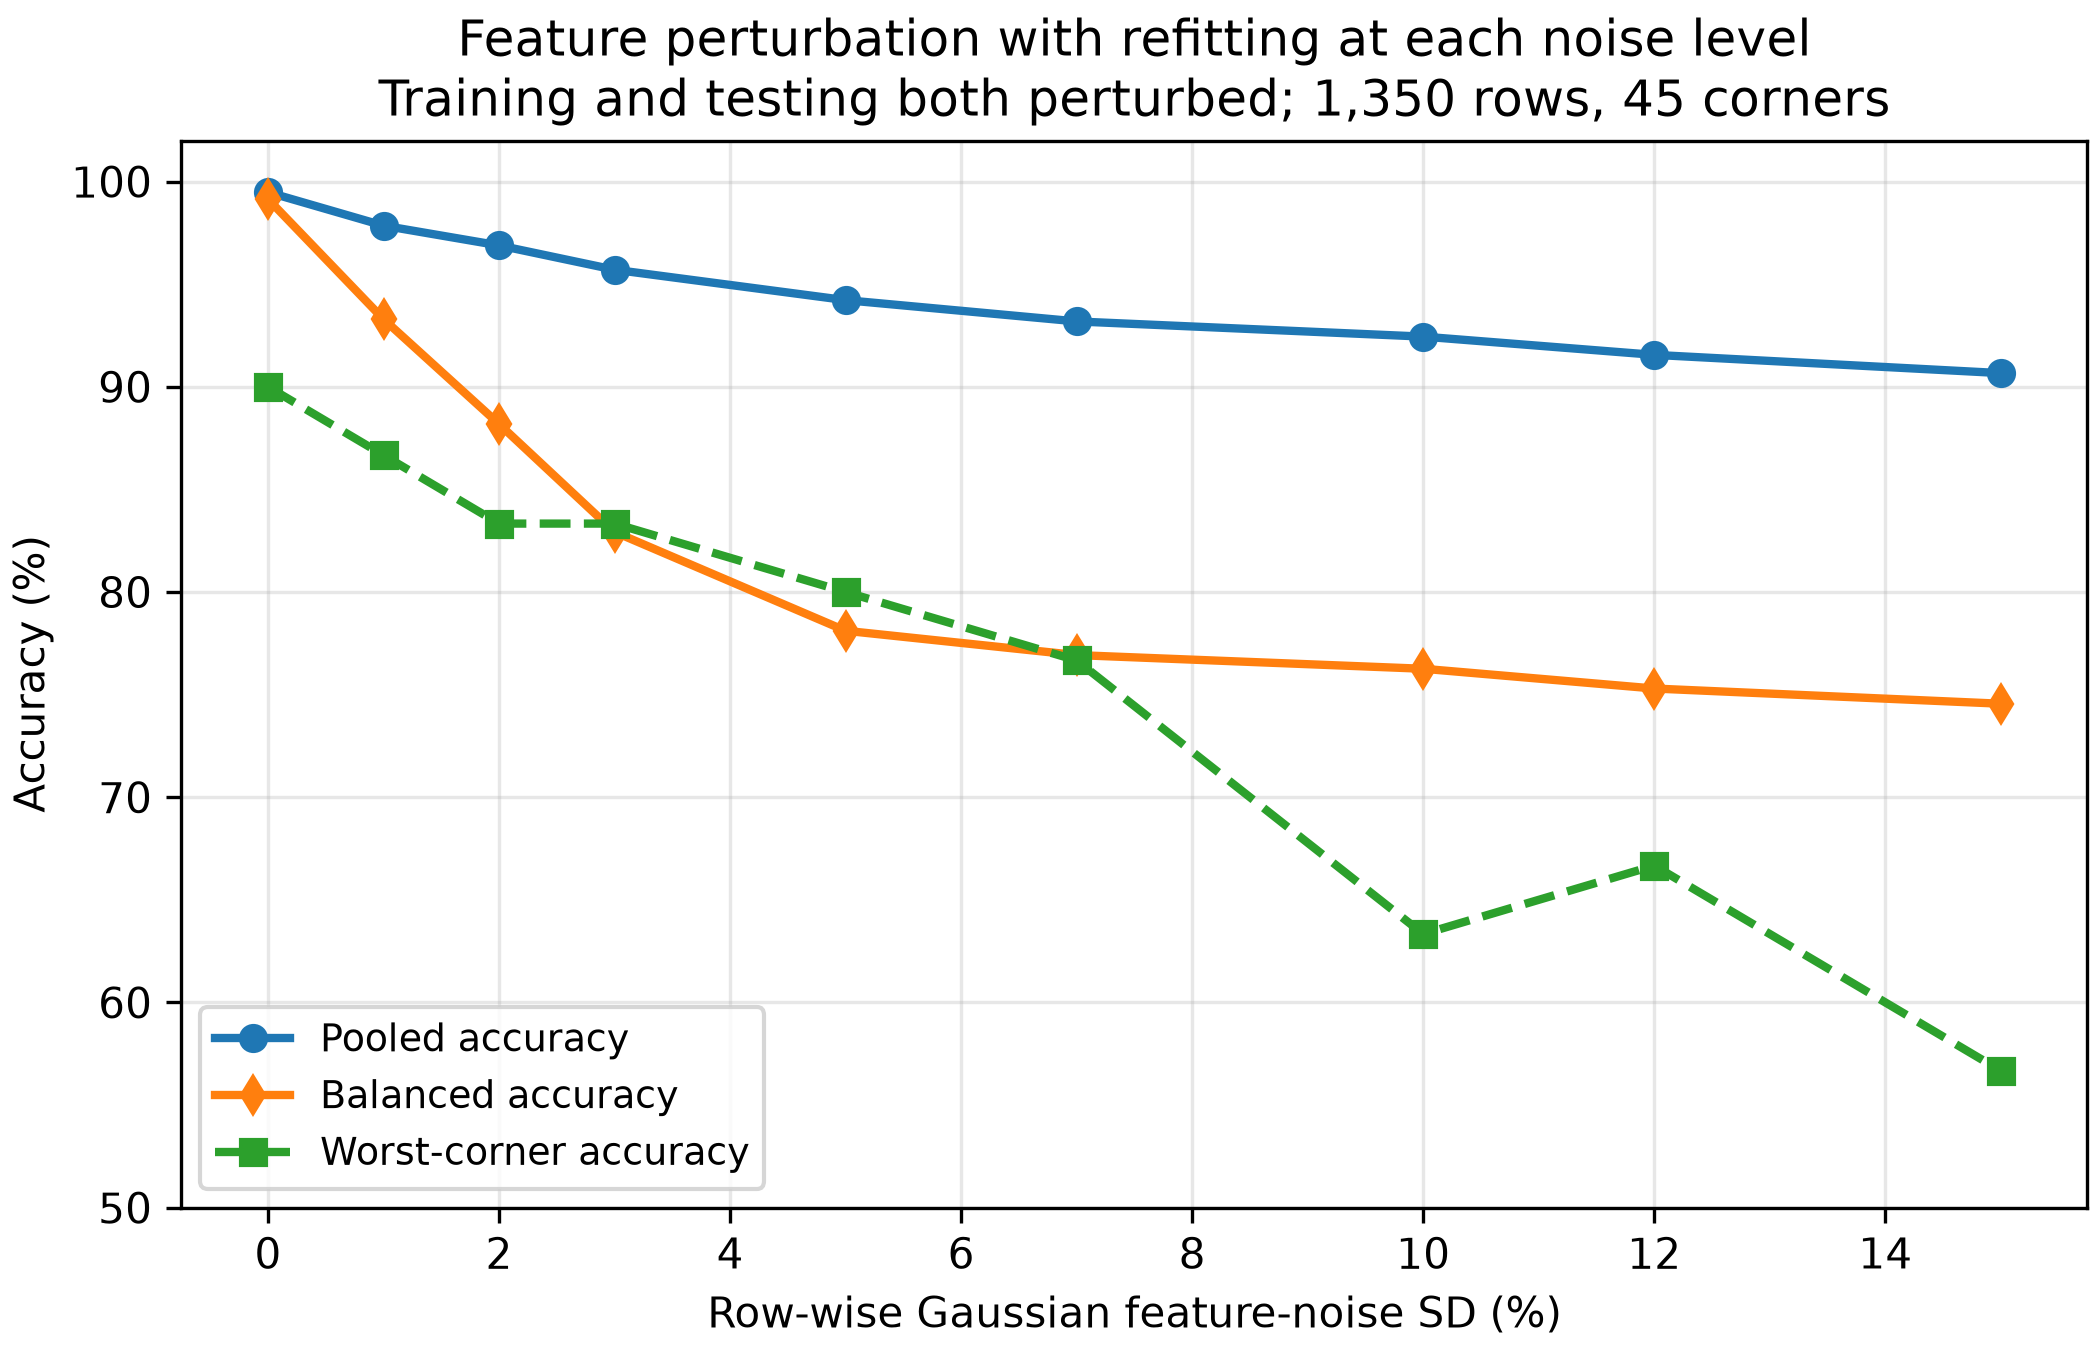
\includegraphics[width=\columnwidth]{fig6_reference_mismatch_sensitivity.png}
\caption{RF accuracy with one shared multiplier per row across the eight ratios. Models are refitted using perturbed training data for each level.}
\label{fig:noise}
\end{figure}

The recurring deterministic configurations and global process shifts limit inference to the sampled grid. A matched reference is assumed available at each held-out corner. Independent healthy and faulty device realizations are needed to estimate false alarms under mismatch. Likewise, the noise experiment describes refitting under shared training and test noise distributions. Evaluating deployment-only reference error would require perturbing the reference measurements at test time while holding the fitted model fixed.

Fallback-coded values can influence both classification and attribution. For example, a large write-delay value can encode a failed extraction. The sampled standby current also varies nonmonotonically with temperature at some fixed supply voltages, motivating settled-current checks before physical leakage interpretation. Calibrated process models, extracted parasitics, and silicon measurements would expand the scope of the benchmark.

Internal-node SNM sweeps and picosecond timing suit simulation and characterization structures that expose analog signals. Array deployment would require a reference-health check and measurement circuitry with characterized resolution, routing, area, and test time. The four screening flags characterize the applied operations. Coverage of a March test sequence remains a separate evaluation.

\clearpage
\section{Conclusion}

Reference normalization reduces cross-corner dispersion of electrical measurements while retaining the signature of a fixed access-path defect. On the 45-corner transistor-level benchmark, the normalized RF achieves 99.33\% pooled accuracy with a 90.00\% worst-corner floor. The matched controls show that ratios can improve RF diagnosis even when raw reference values are already available. The joint holdout supports interpolation within the sampled fault grid, and the weakest-open result identifies a boundary where diagnosis remains difficult.

\IEEEtriggeratref{6}
\begin{thebibliography}{00}

\bibitem{mukhopadhyay2005modeling}
S.~Mukhopadhyay, H.~Mahmoodi, and K.~Roy, ``Modeling of failure probability and statistical design of SRAM array for yield enhancement in nanoscaled CMOS,'' \emph{IEEE Trans. Comput.-Aided Design Integr. Circuits Syst.}, vol.~24, no.~12, pp.~1859--1880, Dec. 2005, doi: 10.1109/TCAD.2005.852295.

\bibitem{mukhopadhyay2007memories}
S.~Mukhopadhyay, Q.~Chen, and K.~Roy, ``Memories in scaled technologies: A review of process induced failures, test methodologies, and fault tolerance,'' in \emph{Proc. IEEE 10th Design and Diagnostics of Electronic Circuits and Systems (DDECS)}, 2007, pp.~1--6, doi: 10.1109/DDECS.2007.4295256.

\bibitem{vandegoor1993march}
A.~J.~van de Goor, ``Using march tests to test SRAMs,'' \emph{IEEE Des. Test Comput.}, vol.~10, no.~1, pp.~8--14, Mar. 1993, doi: 10.1109/54.199799.

\bibitem{vandegoor2000functional}
A.~J.~van de Goor and Z.~Al-Ars, ``Functional memory faults: A formal notation and a taxonomy,'' in \emph{Proc. 18th IEEE VLSI Test Symp. (VTS)}, 2000, pp.~281--289, doi: 10.1109/VTEST.2000.843856.

\bibitem{hamdioui2003dynamic}
S.~Hamdioui, R.~Wadsworth, J.~Delos~Reyes, and A.~J.~van de Goor, ``Importance of dynamic faults for new SRAM technologies,'' in \emph{Proc. 8th IEEE Eur. Test Workshop (ETW)}, 2003, pp.~29--34, doi: 10.1109/ETW.2003.1231665.

\bibitem{pavlov2004sram}
A.~Pavlov, M.~Sachdev, and J.~Pineda~de~Gyvez, ``An SRAM weak cell fault model and a DFT technique with a programmable detection threshold,'' in \emph{Proc. IEEE Int. Test Conf. (ITC)}, 2004, pp.~1006--1015, doi: 10.1109/TEST.2004.1387366.

\bibitem{sabade2004comparison}
S.~S. Sabade and D.~M.~H. Walker, ``Comparison of effectiveness of current ratio and delta-IDDQ tests,'' in \emph{Proc. 17th Int. Conf. VLSI Design}, 2004, pp.~889--894, doi: 10.1109/ICVD.2004.1261043.

\bibitem{seevinck1987static}
E.~Seevinck, F.~J.~List, and J.~Lohstroh, ``Static-noise margin analysis of MOS SRAM cells,'' \emph{IEEE J. Solid-State Circuits}, vol.~SC-22, no.~5, pp.~748--754, Oct. 1987, doi: 10.1109/JSSC.1987.1052809.

\bibitem{makris2018special}
Y.~Makris, A.~Nahar, H.-G.~D.~Stratigopoulos, and M.~Hutner, ``Special session on machine learning: How will machine learning transform test?'' in \emph{Proc. IEEE 36th VLSI Test Symp. (VTS)}, 2018, pp.~1--9, doi: 10.1109/VTS.2018.8368667.

\bibitem{amrouch2022machine}
H.~Amrouch, K.~Chakrabarty, D.~Pfl\"uger, I.~Polian, M.~Sauer, and M.~Sonza~Reorda, ``Machine learning for test, diagnosis, post-silicon validation and yield optimization,'' in \emph{Proc. IEEE Eur. Test Symp. (ETS)}, 2022, pp.~1--6, doi: 10.1109/ETS54262.2022.9810416.

\bibitem{venkatesan2024sram}
C.~Venkatesan, Y.~Nirsanametla, K.~Sharma, and A.~Shrivastava, ``Deep learning based fault detection and classification in SRAM cells with data augmentation,'' in \emph{Proc. 10th Int. Conf. Adv. Comput. Commun. Syst. (ICACCS)}, 2024, pp.~2659--2663, doi: 10.1109/ICACCS60874.2024.10717291.

\bibitem{pedregosa2011scikit}
F.~Pedregosa, G.~Varoquaux, A.~Gramfort, V.~Michel, B.~Thirion, O.~Grisel, M.~Blondel, P.~Prettenhofer, R.~Weiss, V.~Dubourg, and J.~Vanderplas, ``Scikit-learn: Machine learning in Python,'' \emph{J. Mach. Learn. Res.}, vol.~12, pp.~2825--2830, Nov. 2011.

\bibitem{lundberg2017unified}
S.~M.~Lundberg and S.-I.~Lee, ``A unified approach to interpreting model predictions,'' in \emph{Proc. Adv. Neural Inf. Process. Syst. (NeurIPS)}, vol.~30, 2017, pp.~4765--4774.

\end{thebibliography}

\end{document}
